\documentclass[]{article}
\usepackage{lmodern}
\usepackage{amssymb,amsmath}
\usepackage{ifxetex,ifluatex}
\usepackage{fixltx2e} % provides \textsubscript
\ifnum 0\ifxetex 1\fi\ifluatex 1\fi=0 % if pdftex
  \usepackage[T1]{fontenc}
  \usepackage[utf8]{inputenc}
\else % if luatex or xelatex
  \ifxetex
    \usepackage{mathspec}
  \else
    \usepackage{fontspec}
  \fi
  \defaultfontfeatures{Ligatures=TeX,Scale=MatchLowercase}
\fi
% use upquote if available, for straight quotes in verbatim environments
\IfFileExists{upquote.sty}{\usepackage{upquote}}{}
% use microtype if available
\IfFileExists{microtype.sty}{%
\usepackage{microtype}
\UseMicrotypeSet[protrusion]{basicmath} % disable protrusion for tt fonts
}{}
\usepackage[margin=1in]{geometry}
\usepackage{hyperref}
\hypersetup{unicode=true,
            pdftitle={Improving Intergroup Relations Amid Group Conflict - Results},
            pdfauthor={Christopher Grady},
            pdfborder={0 0 0},
            breaklinks=true}
\urlstyle{same}  % don't use monospace font for urls
\usepackage{graphicx,grffile}
\makeatletter
\def\maxwidth{\ifdim\Gin@nat@width>\linewidth\linewidth\else\Gin@nat@width\fi}
\def\maxheight{\ifdim\Gin@nat@height>\textheight\textheight\else\Gin@nat@height\fi}
\makeatother
% Scale images if necessary, so that they will not overflow the page
% margins by default, and it is still possible to overwrite the defaults
% using explicit options in \includegraphics[width, height, ...]{}
\setkeys{Gin}{width=\maxwidth,height=\maxheight,keepaspectratio}
\IfFileExists{parskip.sty}{%
\usepackage{parskip}
}{% else
\setlength{\parindent}{0pt}
\setlength{\parskip}{6pt plus 2pt minus 1pt}
}
\setlength{\emergencystretch}{3em}  % prevent overfull lines
\providecommand{\tightlist}{%
  \setlength{\itemsep}{0pt}\setlength{\parskip}{0pt}}
\setcounter{secnumdepth}{5}
% Redefines (sub)paragraphs to behave more like sections
\ifx\paragraph\undefined\else
\let\oldparagraph\paragraph
\renewcommand{\paragraph}[1]{\oldparagraph{#1}\mbox{}}
\fi
\ifx\subparagraph\undefined\else
\let\oldsubparagraph\subparagraph
\renewcommand{\subparagraph}[1]{\oldsubparagraph{#1}\mbox{}}
\fi

%%% Use protect on footnotes to avoid problems with footnotes in titles
\let\rmarkdownfootnote\footnote%
\def\footnote{\protect\rmarkdownfootnote}

%%% Change title format to be more compact
\usepackage{titling}

% Create subtitle command for use in maketitle
\providecommand{\subtitle}[1]{
  \posttitle{
    \begin{center}\large#1\end{center}
    }
}

\setlength{\droptitle}{-2em}

  \title{Improving Intergroup Relations Amid Group Conflict - Results}
    \pretitle{\vspace{\droptitle}\centering\huge}
  \posttitle{\par}
    \author{Christopher Grady}
    \preauthor{\centering\large\emph}
  \postauthor{\par}
      \predate{\centering\large\emph}
  \postdate{\par}
    \date{December 09, 2019}

\usepackage{float}

\begin{document}
\maketitle

\hypertarget{results}{%
\section{Results}\label{results}}

Our major finding is that the program improved intergroup attitudes,
spurred intergroup contact outside of the program, and reduced feelings
of insecurity. The program had the largest impact on respondents who
participated on ECPN committees, but the effect extended to respondents
who did not participate with ECPN. We use coefficient plots to report
average treatment effects in our community-level data and in our
individual-level data. We also use coefficient plots to show differences
between participants, nonparticipants, and controls in our
individual-level data. All coefficient plots show bootstrapped 95\%
confidence intervals and standardized coefficients.

Figure 1 and 2 shows ECPN's effect on outcomes. Figure 1 shows the main
analyses, where the solid lines are the community-level data and the
dashed lines are the individual-level data. Figure 2 shows participants
and nonparticipants compared to controls.

\begin{figure}[!h]
    \begin{minipage}[b]{.48\textwidth}
        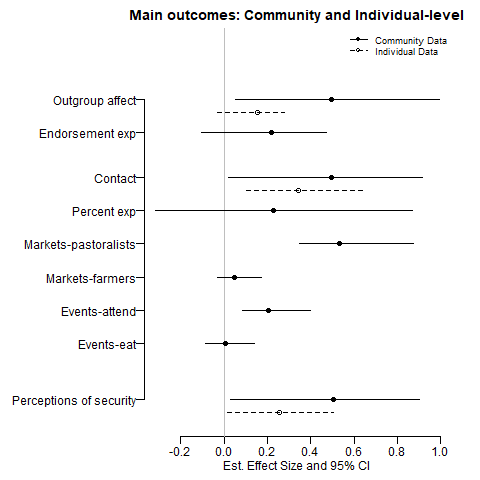
\includegraphics[width=\linewidth]{../figs/ecpn_coefplots_MainOuts-cats.png}
        %\caption{Look at fig 1!}
        \label{fig:fig1}
    \end{minipage}
    \hfill
    \begin{minipage}[b]{.48\textwidth}
        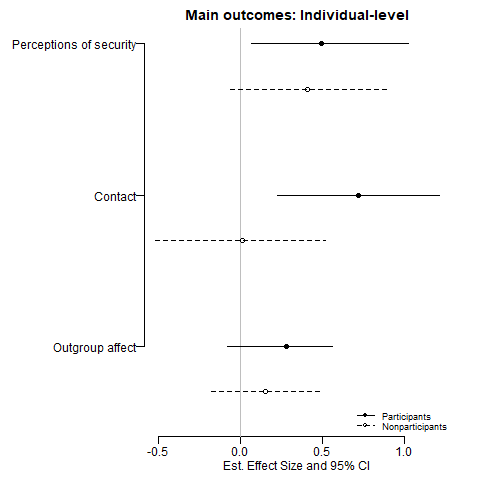
\includegraphics[width=\linewidth]{../figs/ecpn_coefplots_MainOuts_panel-cats.png}
        %\caption{Look at fig 2!}
        \label{fig:fig2}
    \end{minipage}
\end{figure}

\hypertarget{intergroup-affect}{%
\subsection{Intergroup Affect}\label{intergroup-affect}}

ECPN bolstered intergroup affect in treatment communities. Respondents
in treatment communities report more trust the other group and are more
comfortable engaging in various relationships with the outgroup, such as
trading goods and intermarriage. Intergroup affect as measured by the
endorsement experiment also improves more in the treatment group than
the control group, though the difference is not statistically
significant at conventional levels.

Figures 3 and 4 show the effect of ECPN on the intergroup affect survey
index. Descriptively, affect in control communities decreased from
baseline to endline, while intervention communities improved over the
same time period. As measured by the endorsement experiment, affect
declines in both treatment and control communities, but declines more in
control communities. Both measures suggest that ECPN improved affect
towards the outgroup.

\begin{figure}[!h]
    \begin{minipage}[b]{.48\textwidth}
        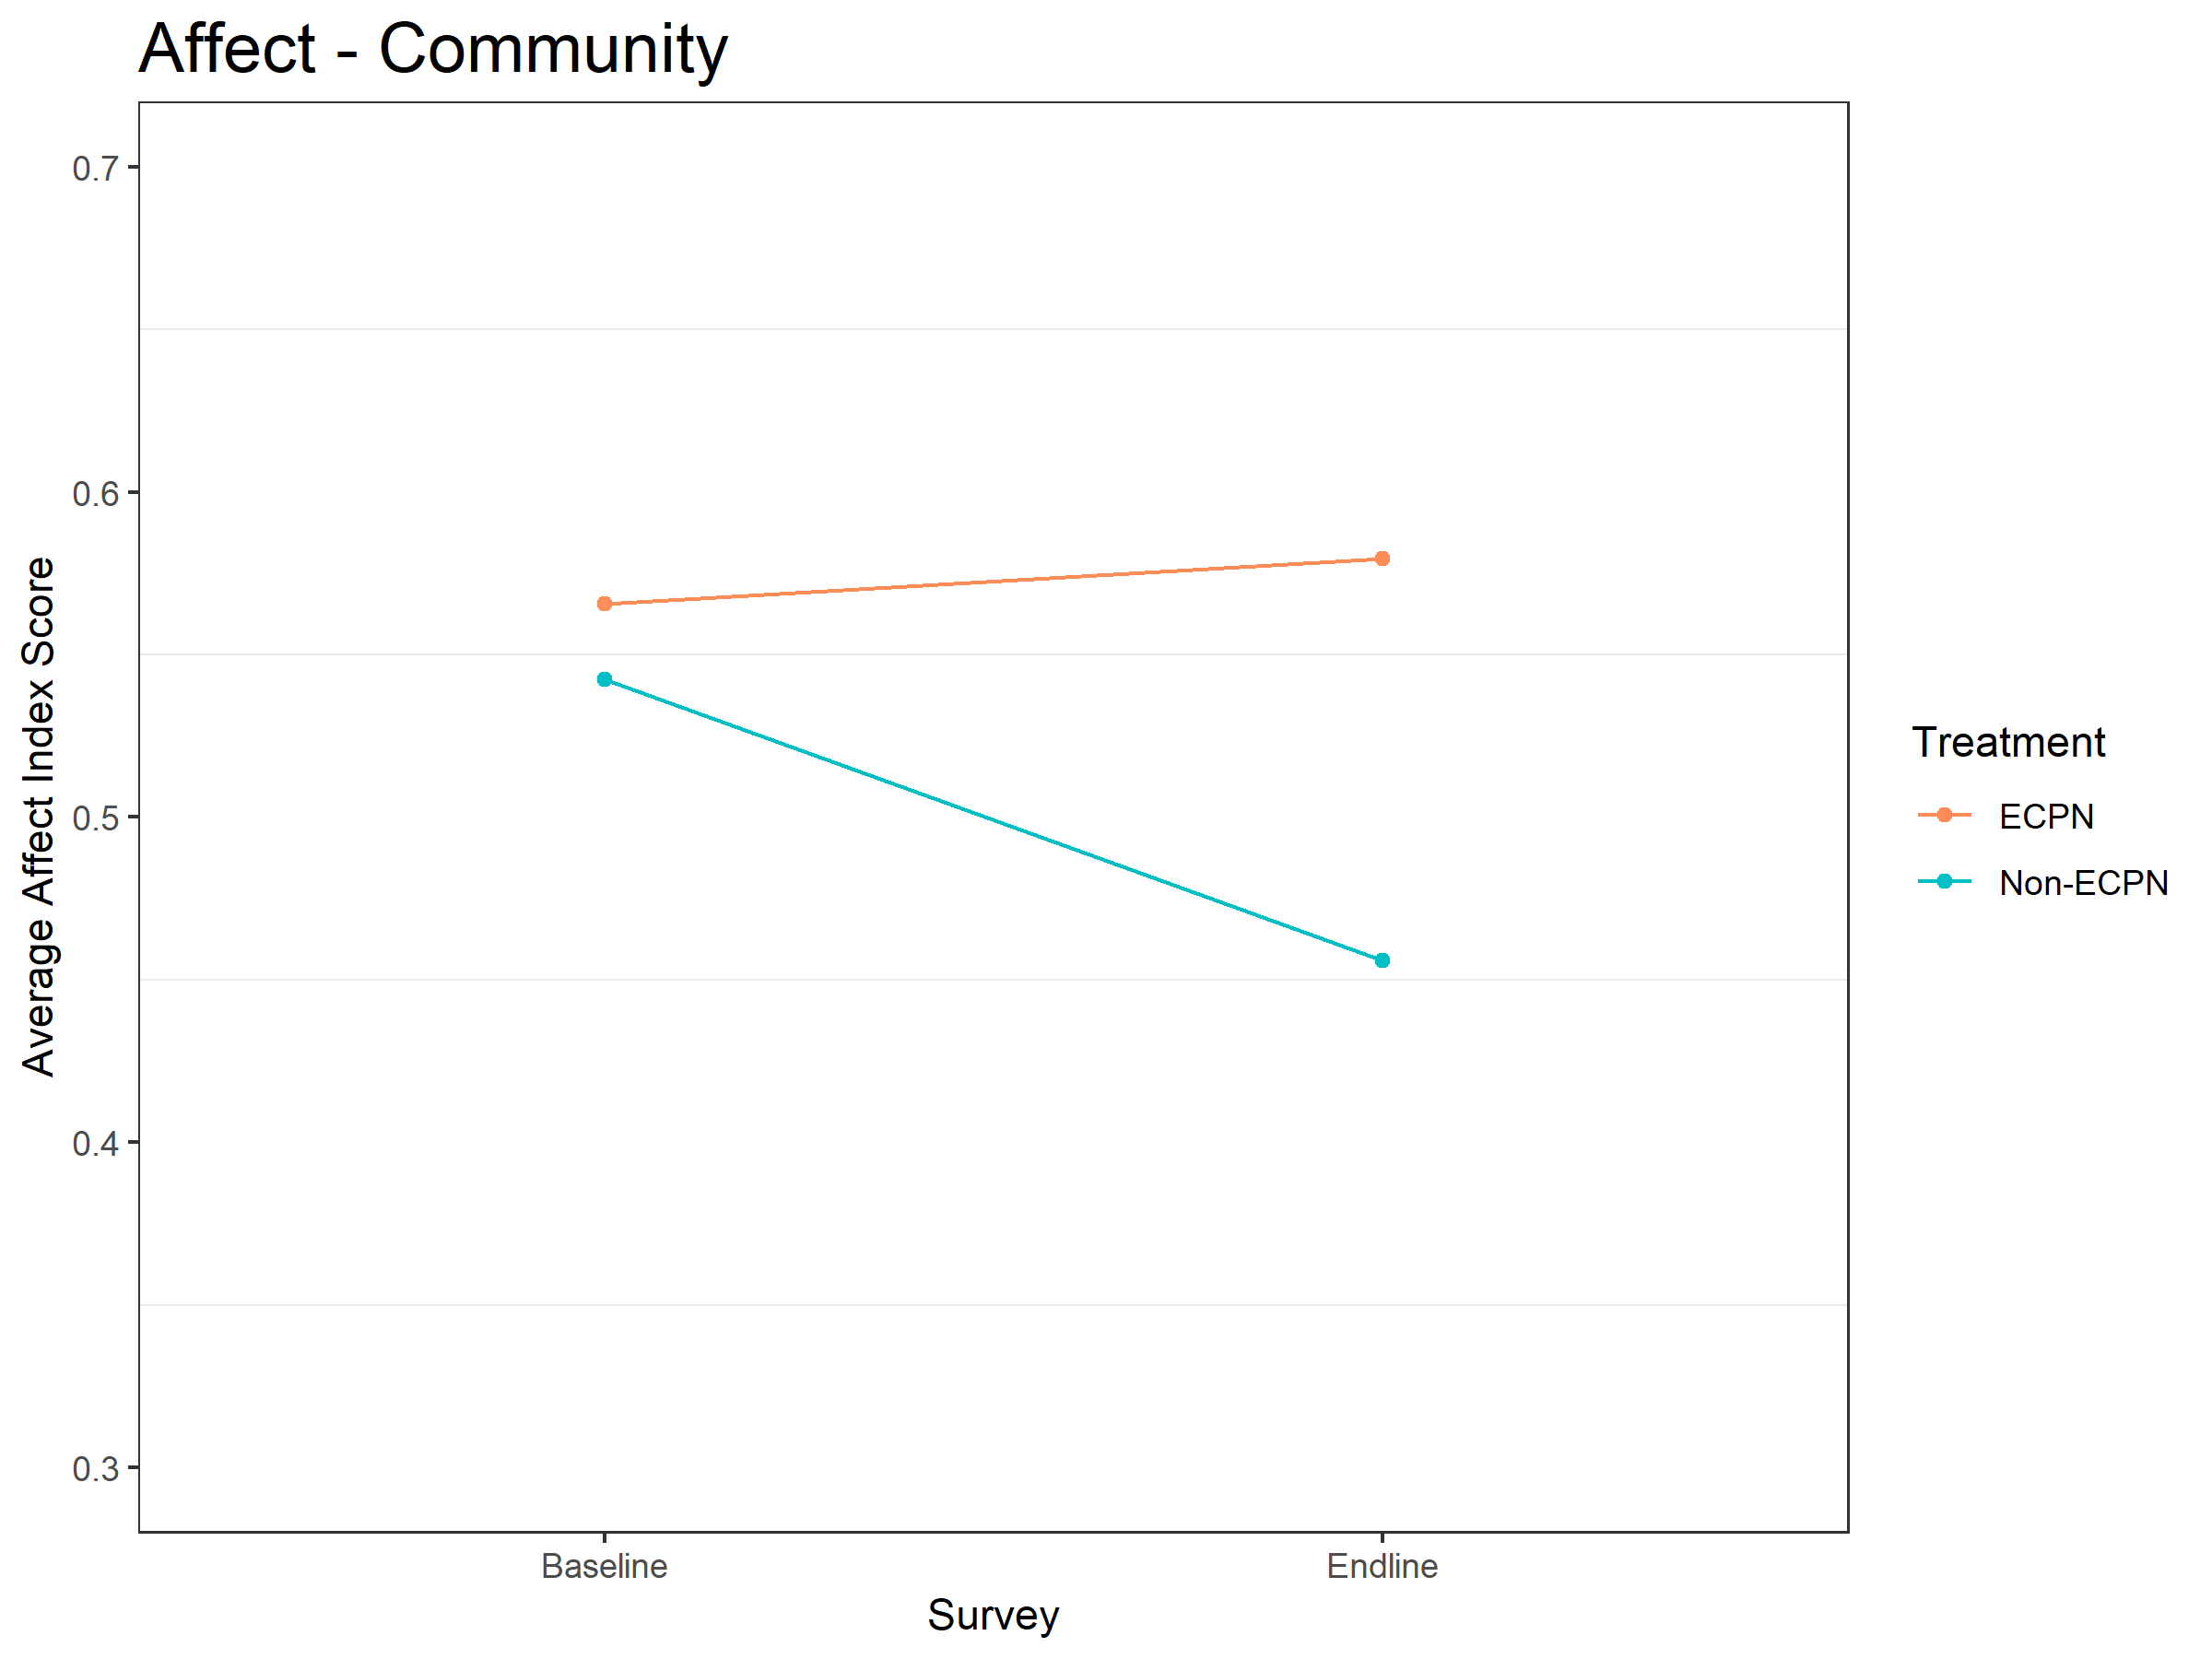
\includegraphics[width=\linewidth]{../figs/affectComm_plot.png}
        %\caption{Look at fig 1!}
        \label{fig:fig3}
    \end{minipage}
    \hfill
    \begin{minipage}[b]{.48\textwidth}
        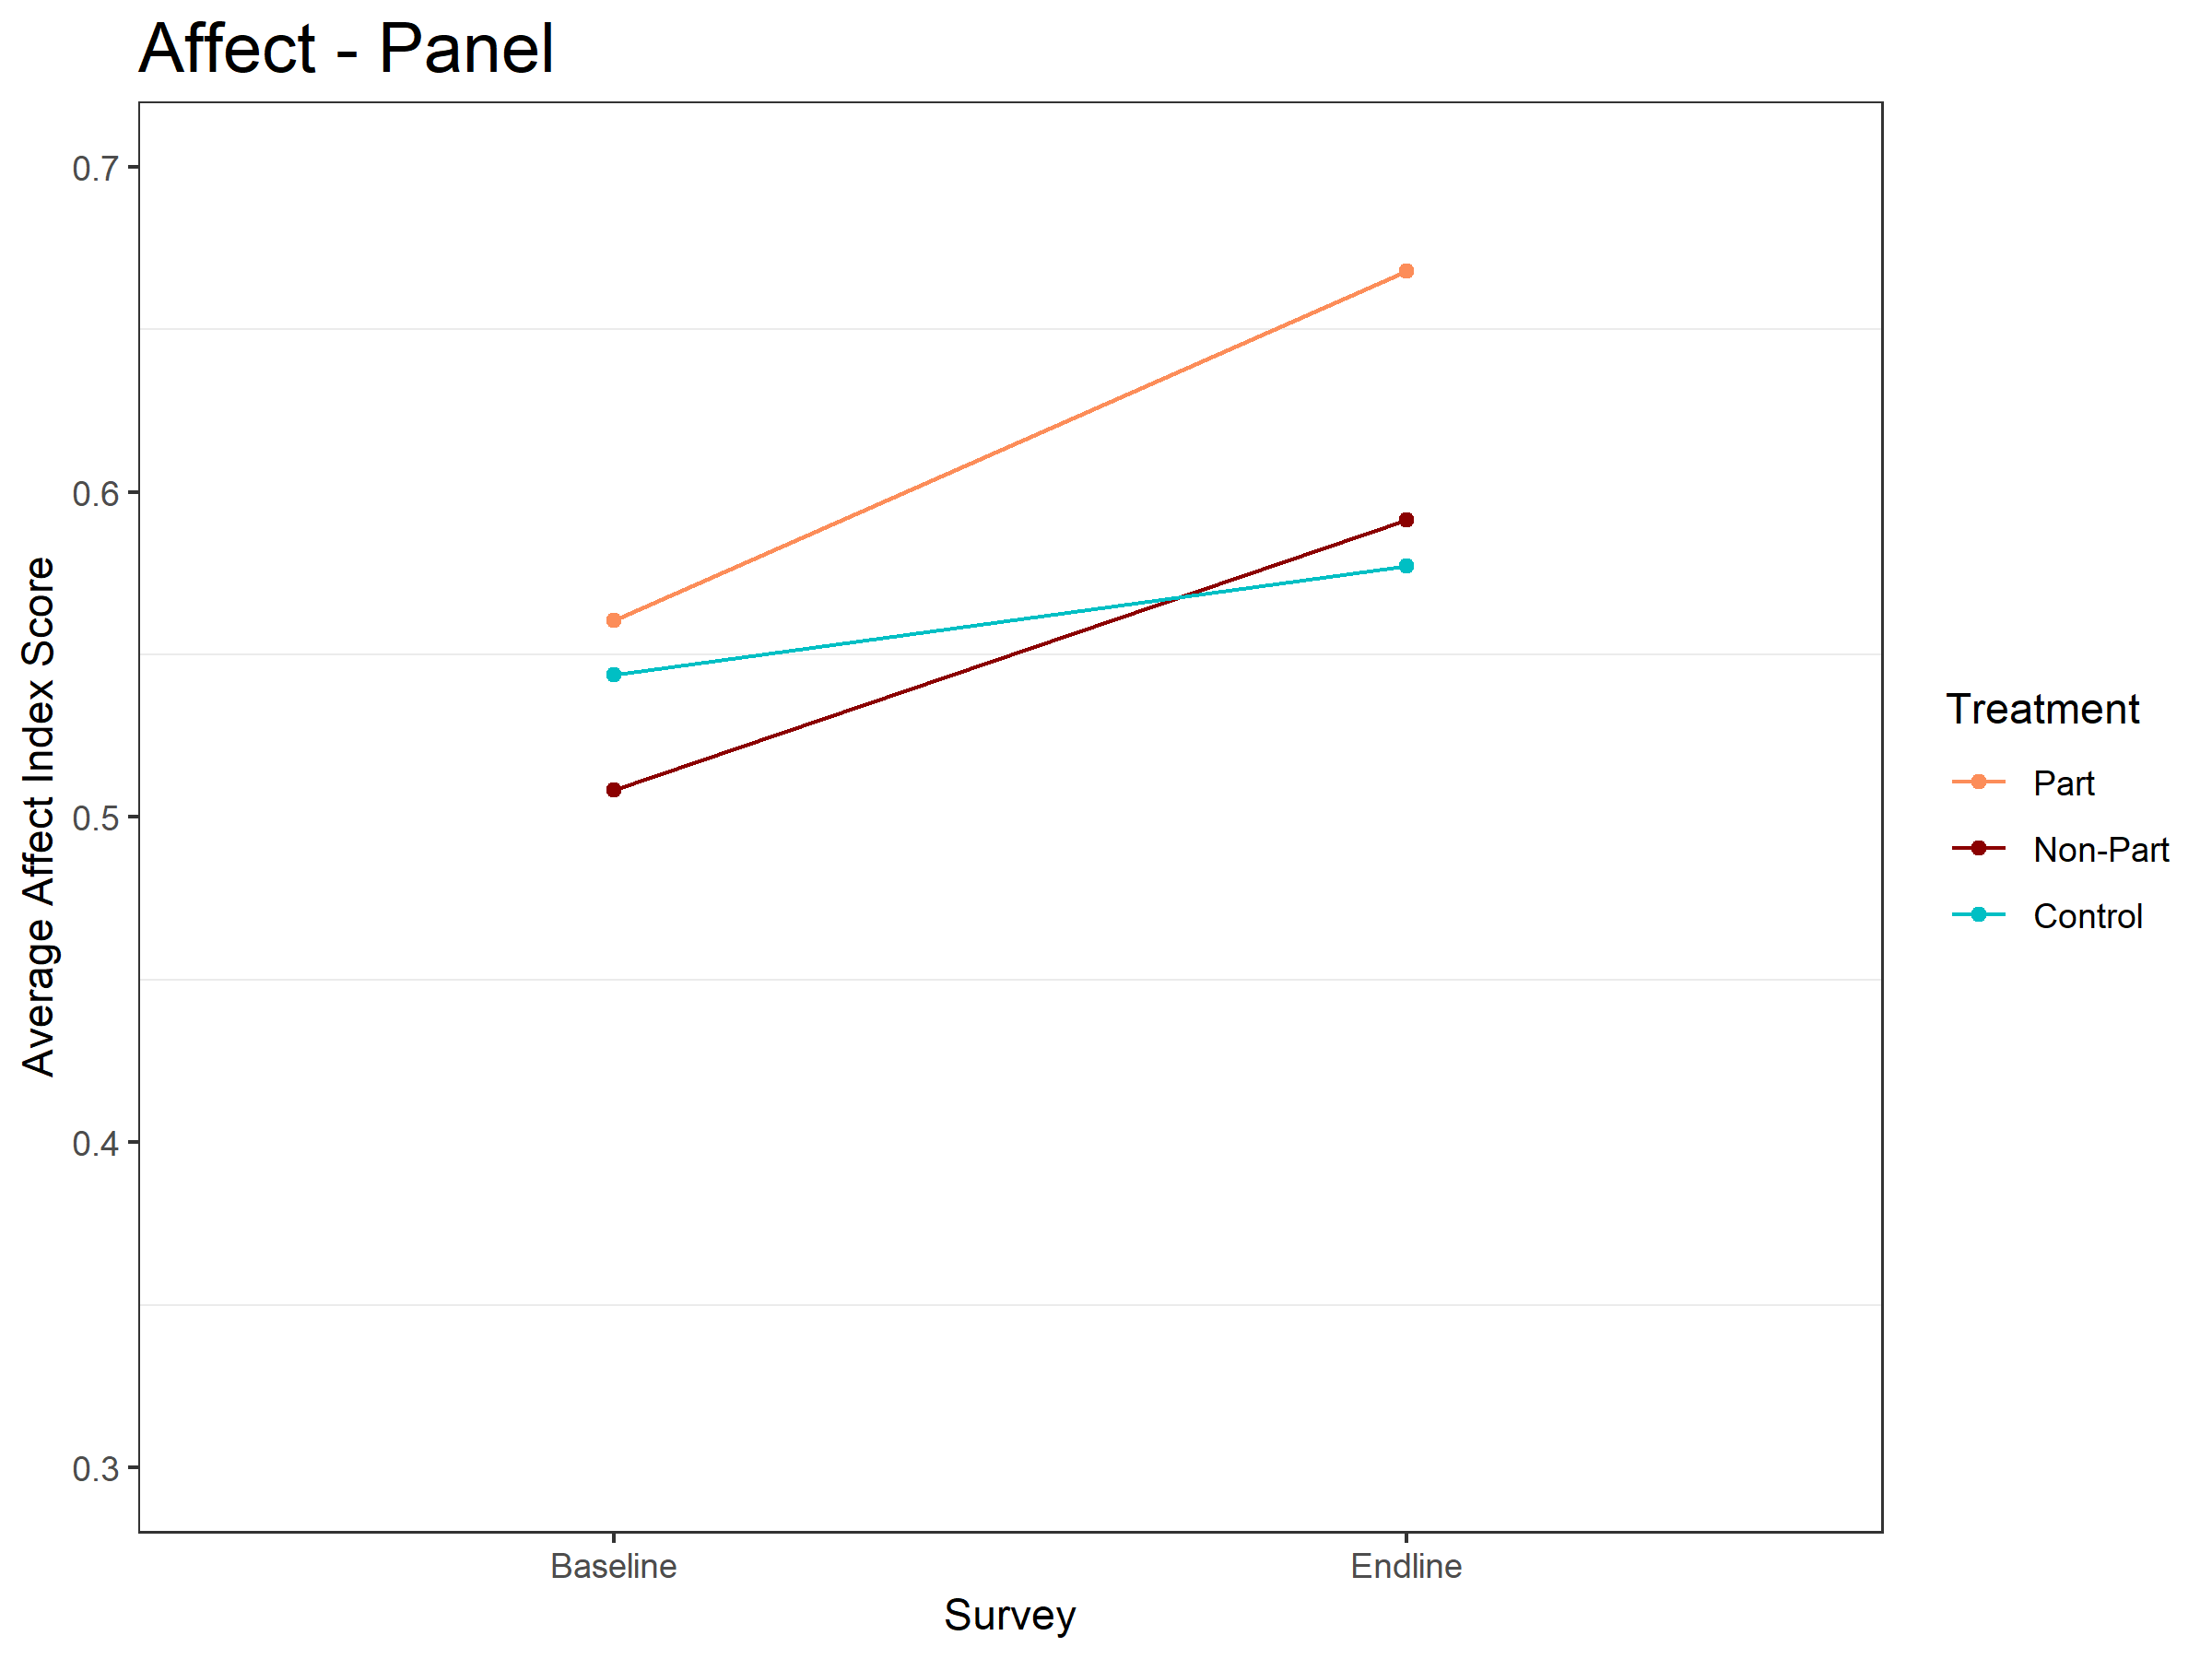
\includegraphics[width=\linewidth]{../figs/affectPan_plot.png}
        %\caption{Look at fig 2!}
        \label{fig:fig4}
    \end{minipage}
\end{figure}

\hypertarget{contact}{%
\subsection{Contact}\label{contact}}

The effect of ECPN on contact is substantial. Respondents in treatment
communities report more contact and more willingness to engage in
contact at all levels of the percent experiment; we also observe more
pastoralists in markets interacting with farmers. Since the markets are
all located in the farming community, the sustained presence of
pastoralists there suggests that (1) farmers were accepting/tolerant of
pastoralists in their community and (2) pastoralists felt comfortable
spending time in the farmer community. The number of farmers present in
the markets does not change in either group, which makes sense because
the market is inside the farming community.

\begin{figure}[!h]
    \begin{minipage}[b]{.48\textwidth}
        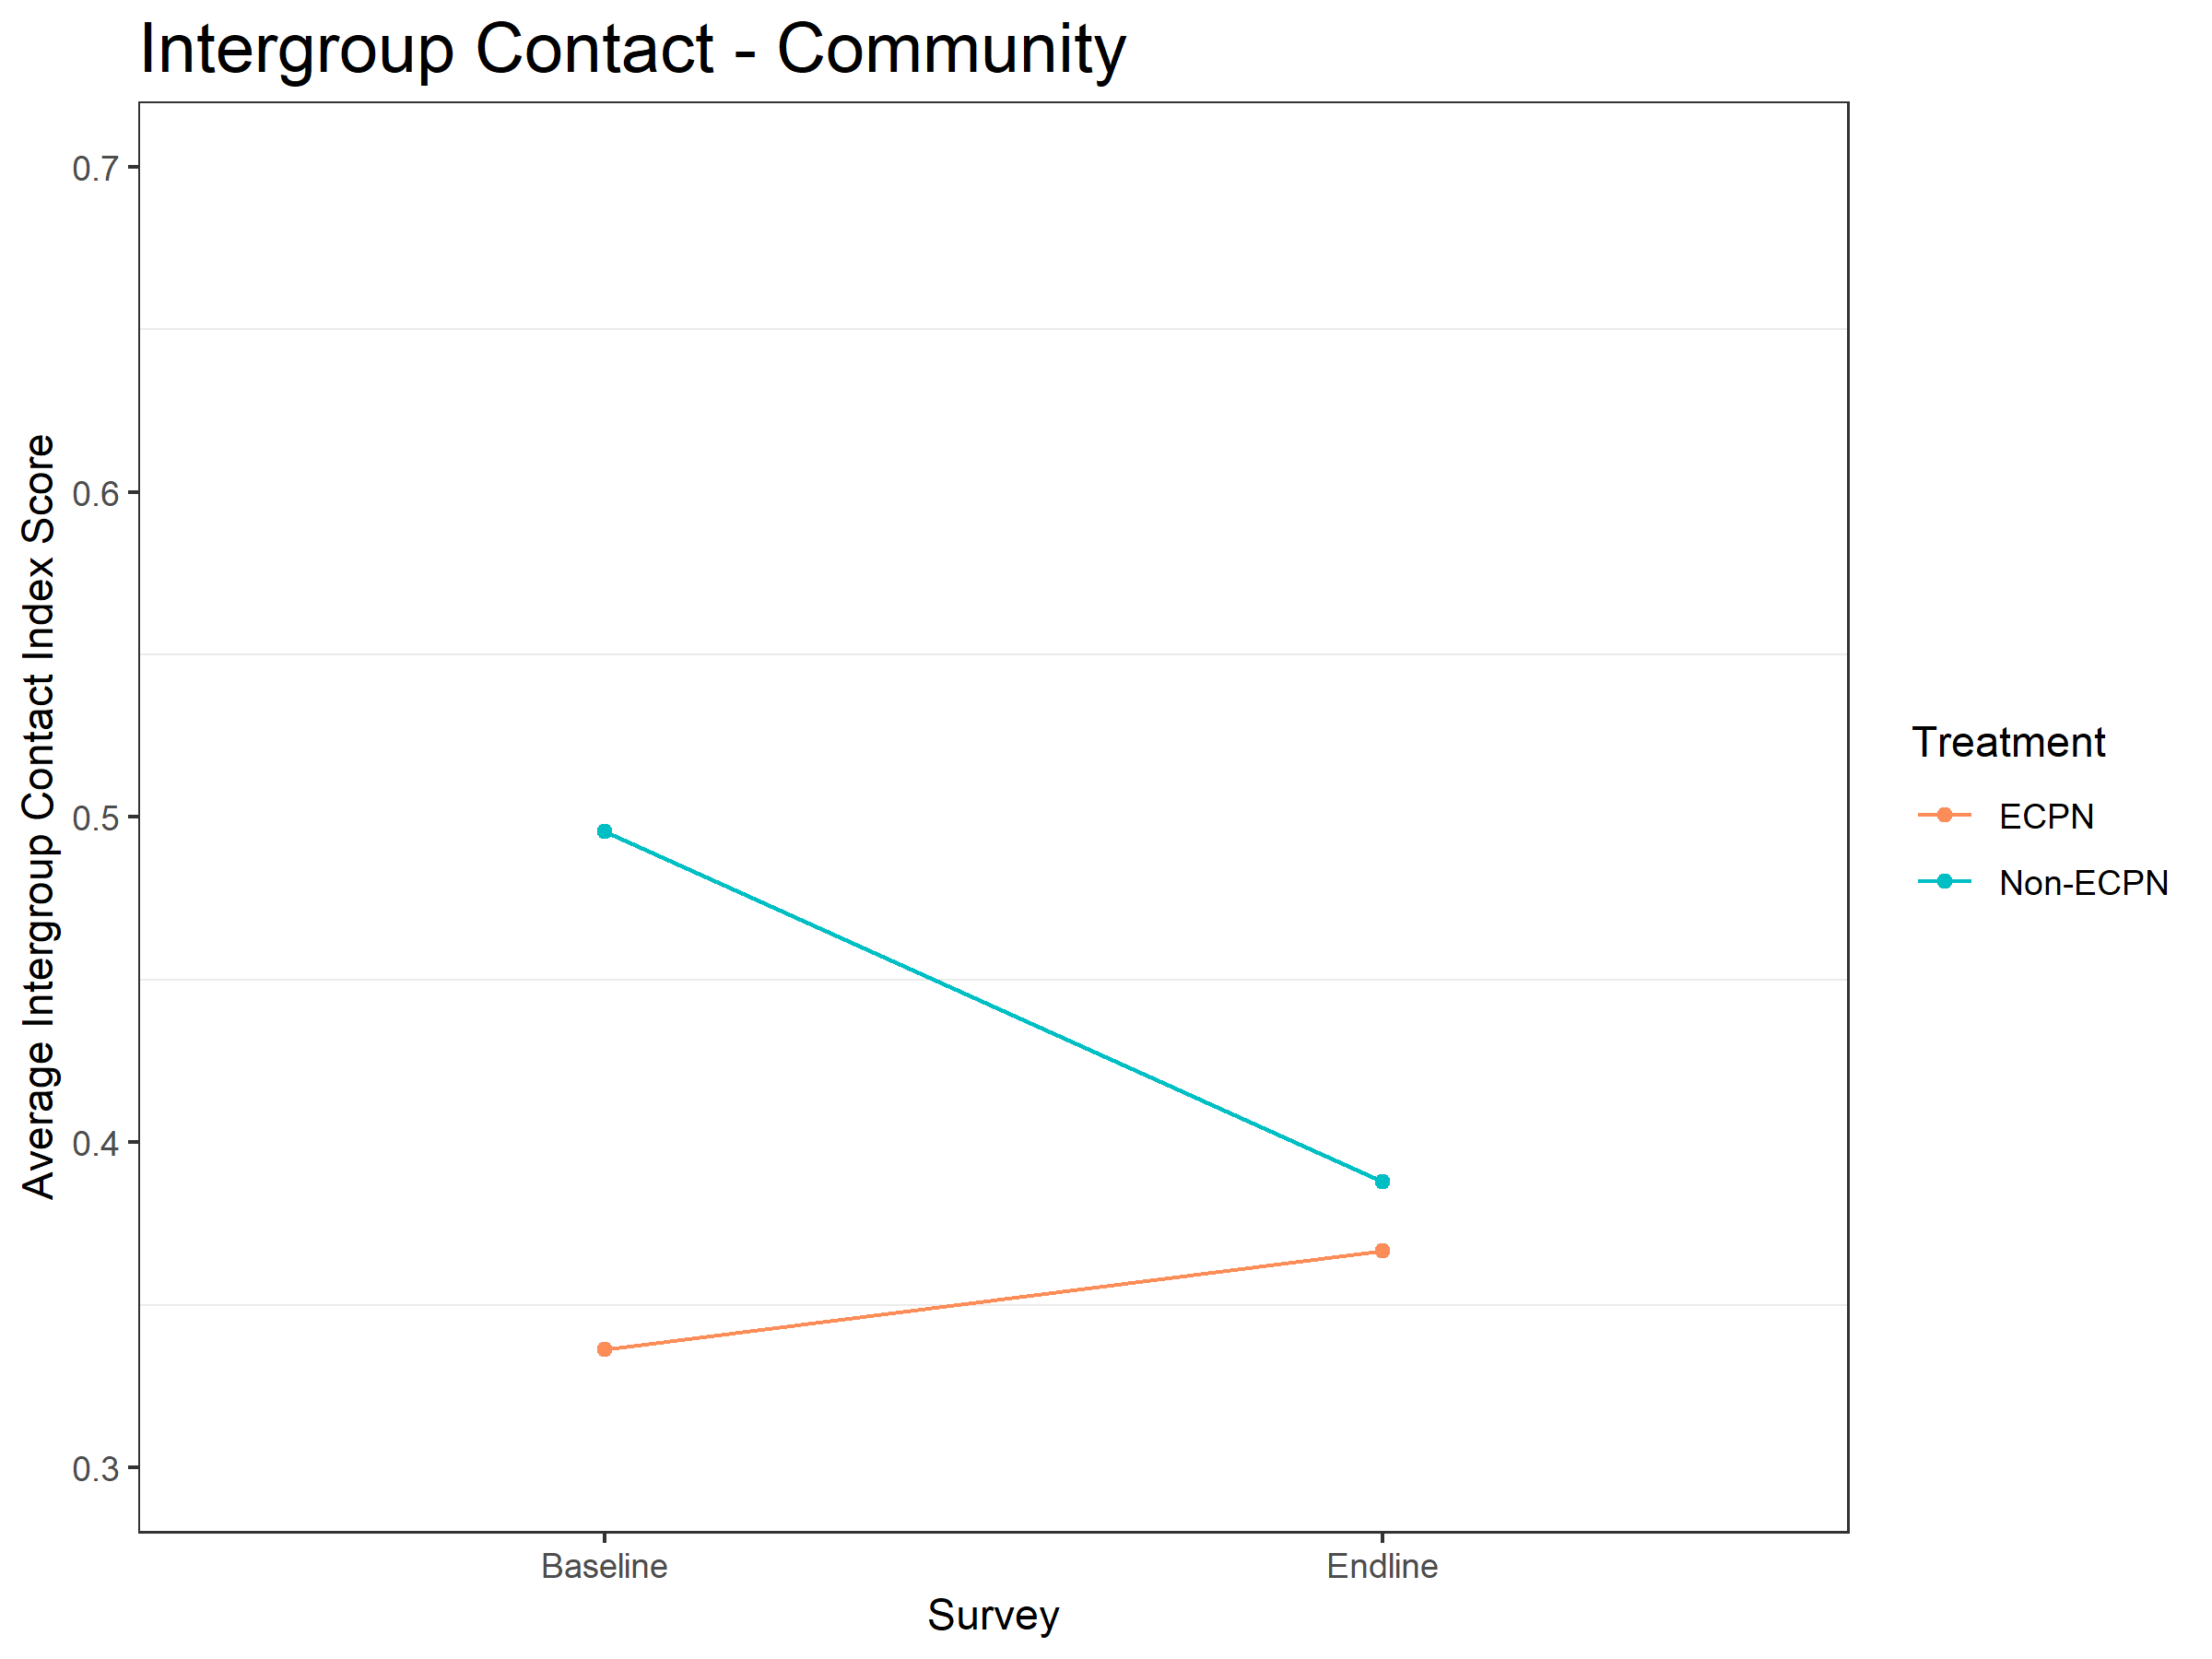
\includegraphics[width=\linewidth]{../figs/conComm_plot.png}
        %\caption{Look at fig 1!}
        \label{fig:fig5}
    \end{minipage}
    \hfill
    \begin{minipage}[b]{.48\textwidth}
        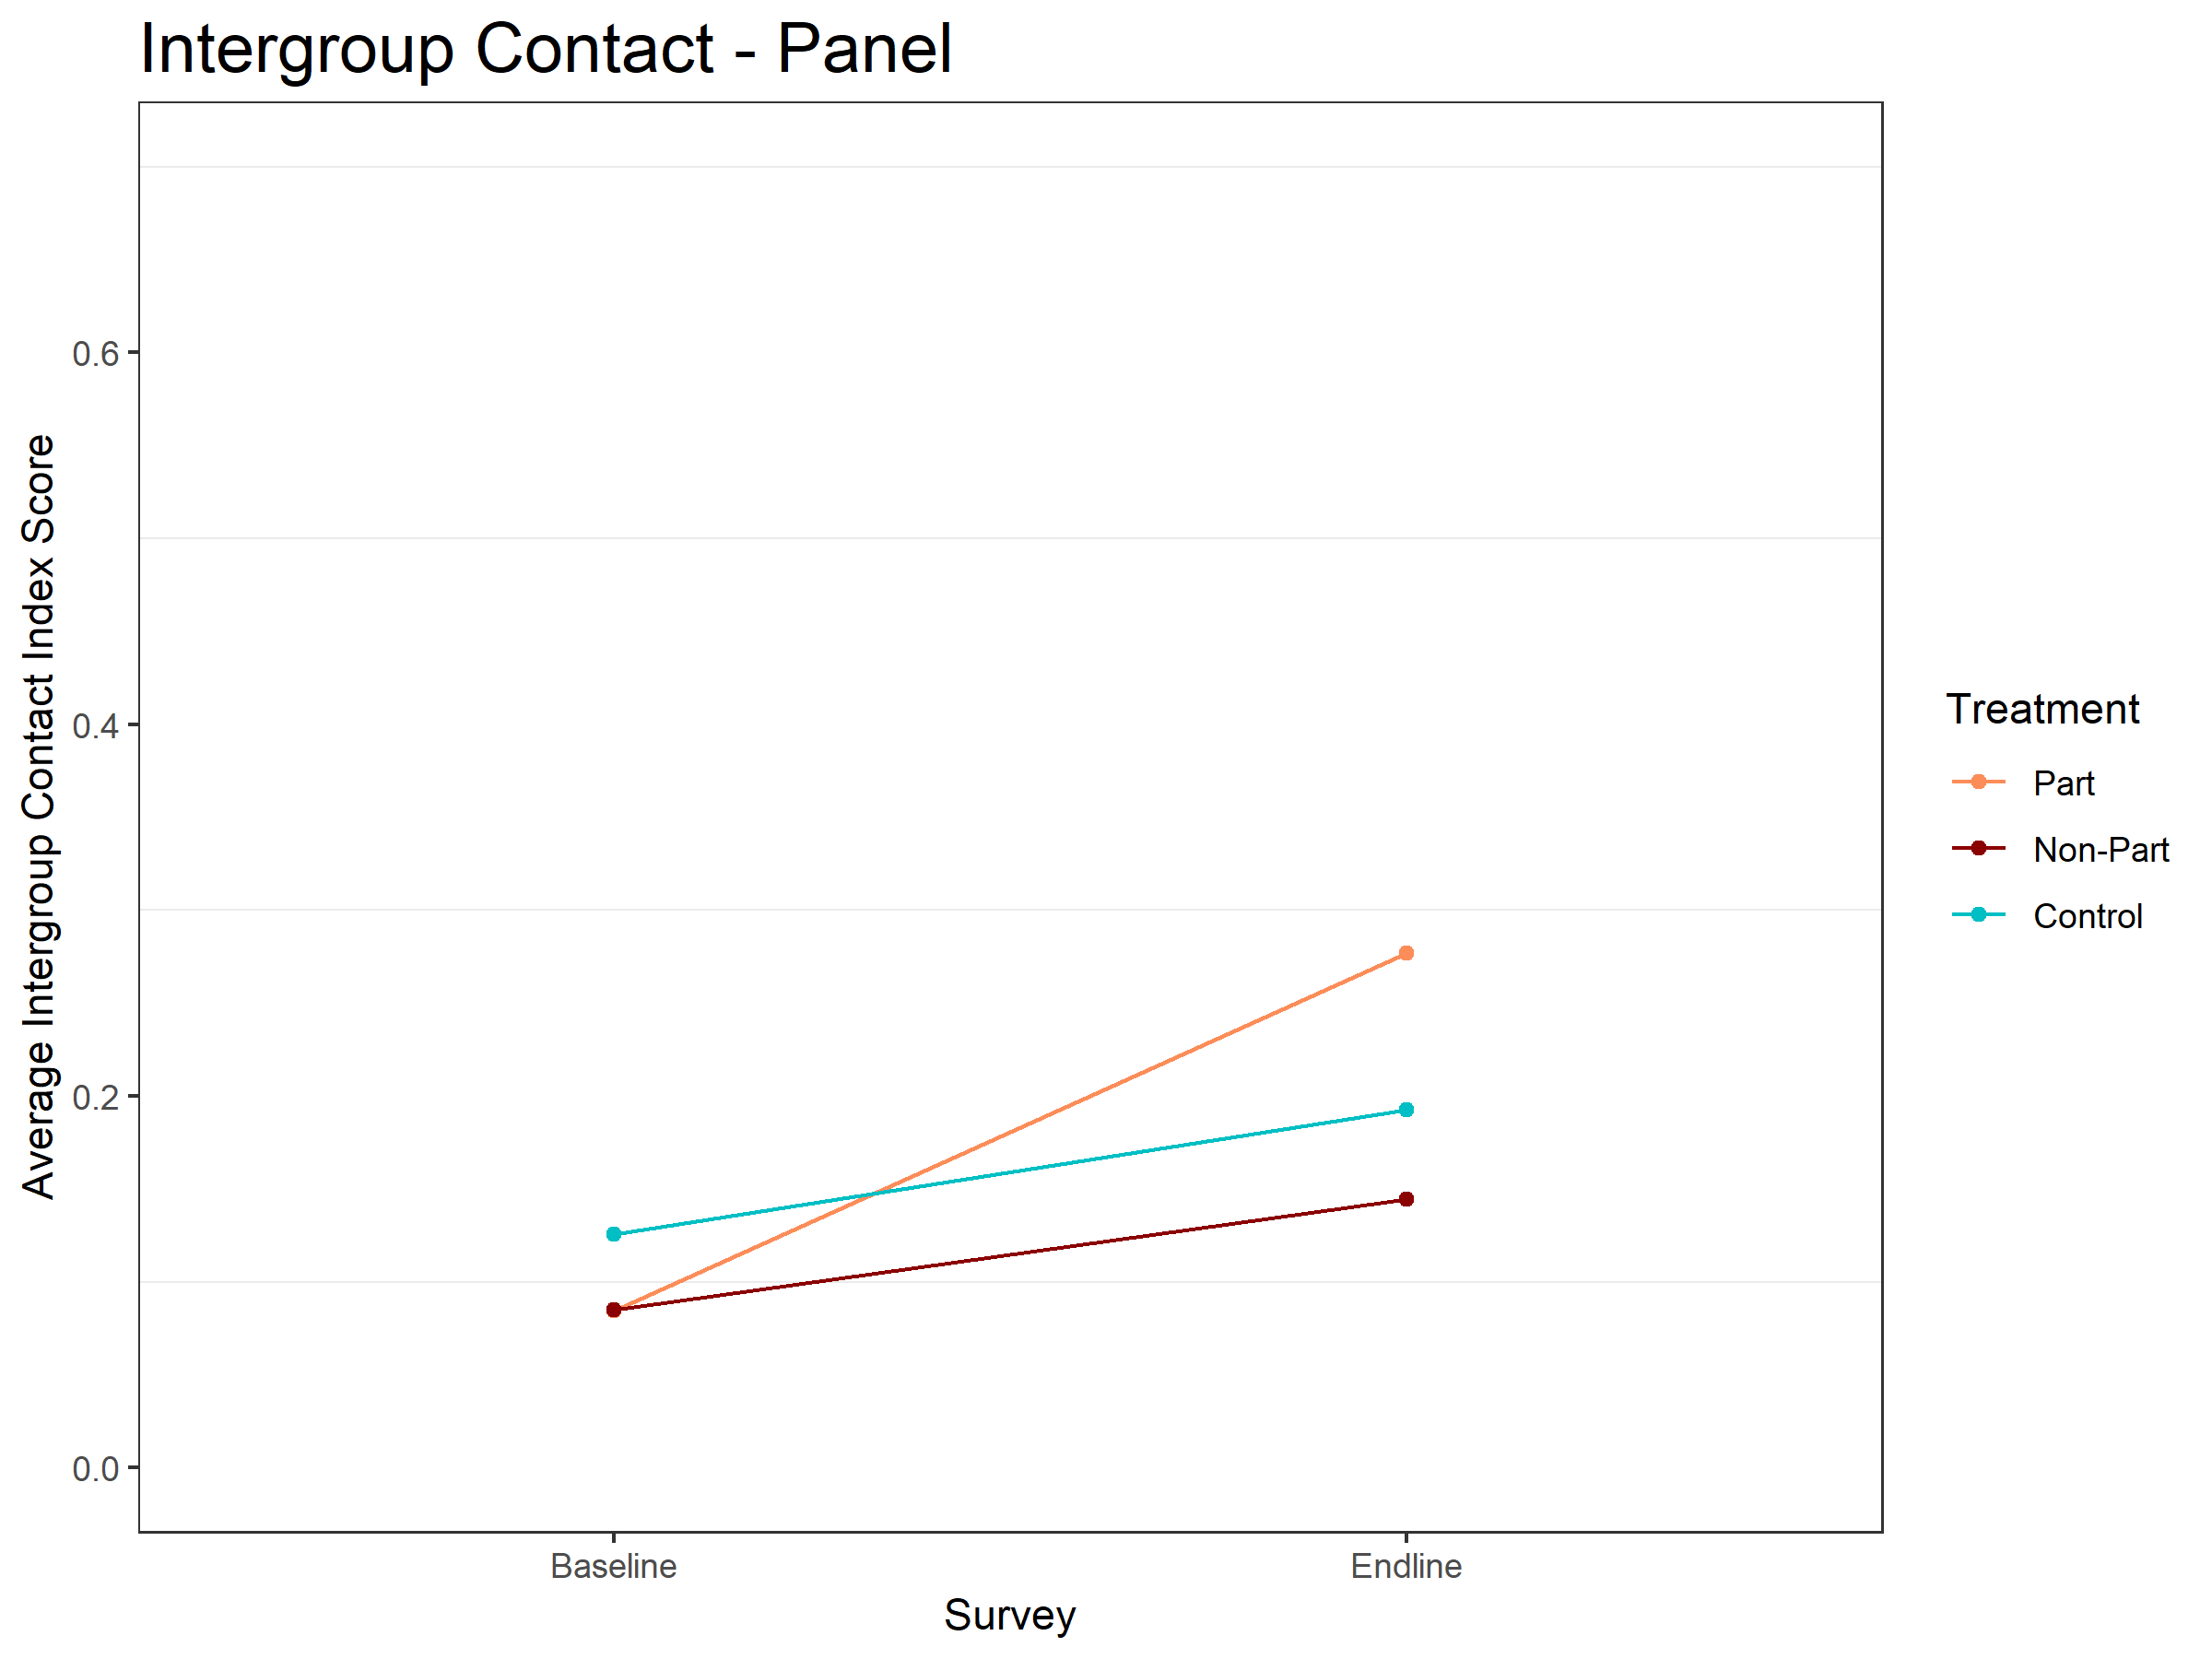
\includegraphics[width=\linewidth]{../figs/conPan_plot.png}
        %\caption{Look at fig 2!}
        \label{fig:fig6}
    \end{minipage}
\end{figure}

Figures 5 and 6 shows the effect of ECPN on the contact survey outcomes.
Descriptively, the community-level self-reports show that intergroup
contact declined sharply in control communities but rose slightly in
treatment communities. It is impressive that ECPN increased contact
while the social environment led to a sharp decline in control sites.
The secular decline is due to the displacement in Benue, where
intergroup contact went down for every group, though it declined far
less in treatment sites. In Nasarawa, intergroup contact increased in
both treatment and control sites, but far more in treatment sites.

At the individual-level, intergroup contact increased for committee
participants but stayed largely the same for nonparticipants and
controls. The large community-level effect, however, suggests that the
effects of ECPN \emph{did} extend to nonparticipants in treatment
comunities. But the effect did not extend to the type of nonparticipant
who we could track down and resurvey.

\hypertarget{insecurity}{%
\subsection{Insecurity}\label{insecurity}}

ECPN's substantially decreased feelings of insecurity in the treatment
group. The effect is large in both the community-level and the
individual-level data. Security in ECPN communities improved far more
from baseline to endline than in control communities. At the
individual-level, participants and nonparticipants improved equally,
suggesting that these increases reflect a change in the conflict
environment that impacts the entire community, not just respondents
involved in ECPN committees. These improvements in treatment communities
are especially powerful because other survey questions show that ECPN
increased awareness of the conflict -- respondents in ECPN communities
are more likely than the control to know that violence between groups
has occurred recently, yet they feel more secure.

\begin{figure}[!h]
    \begin{minipage}[b]{.48\textwidth}
        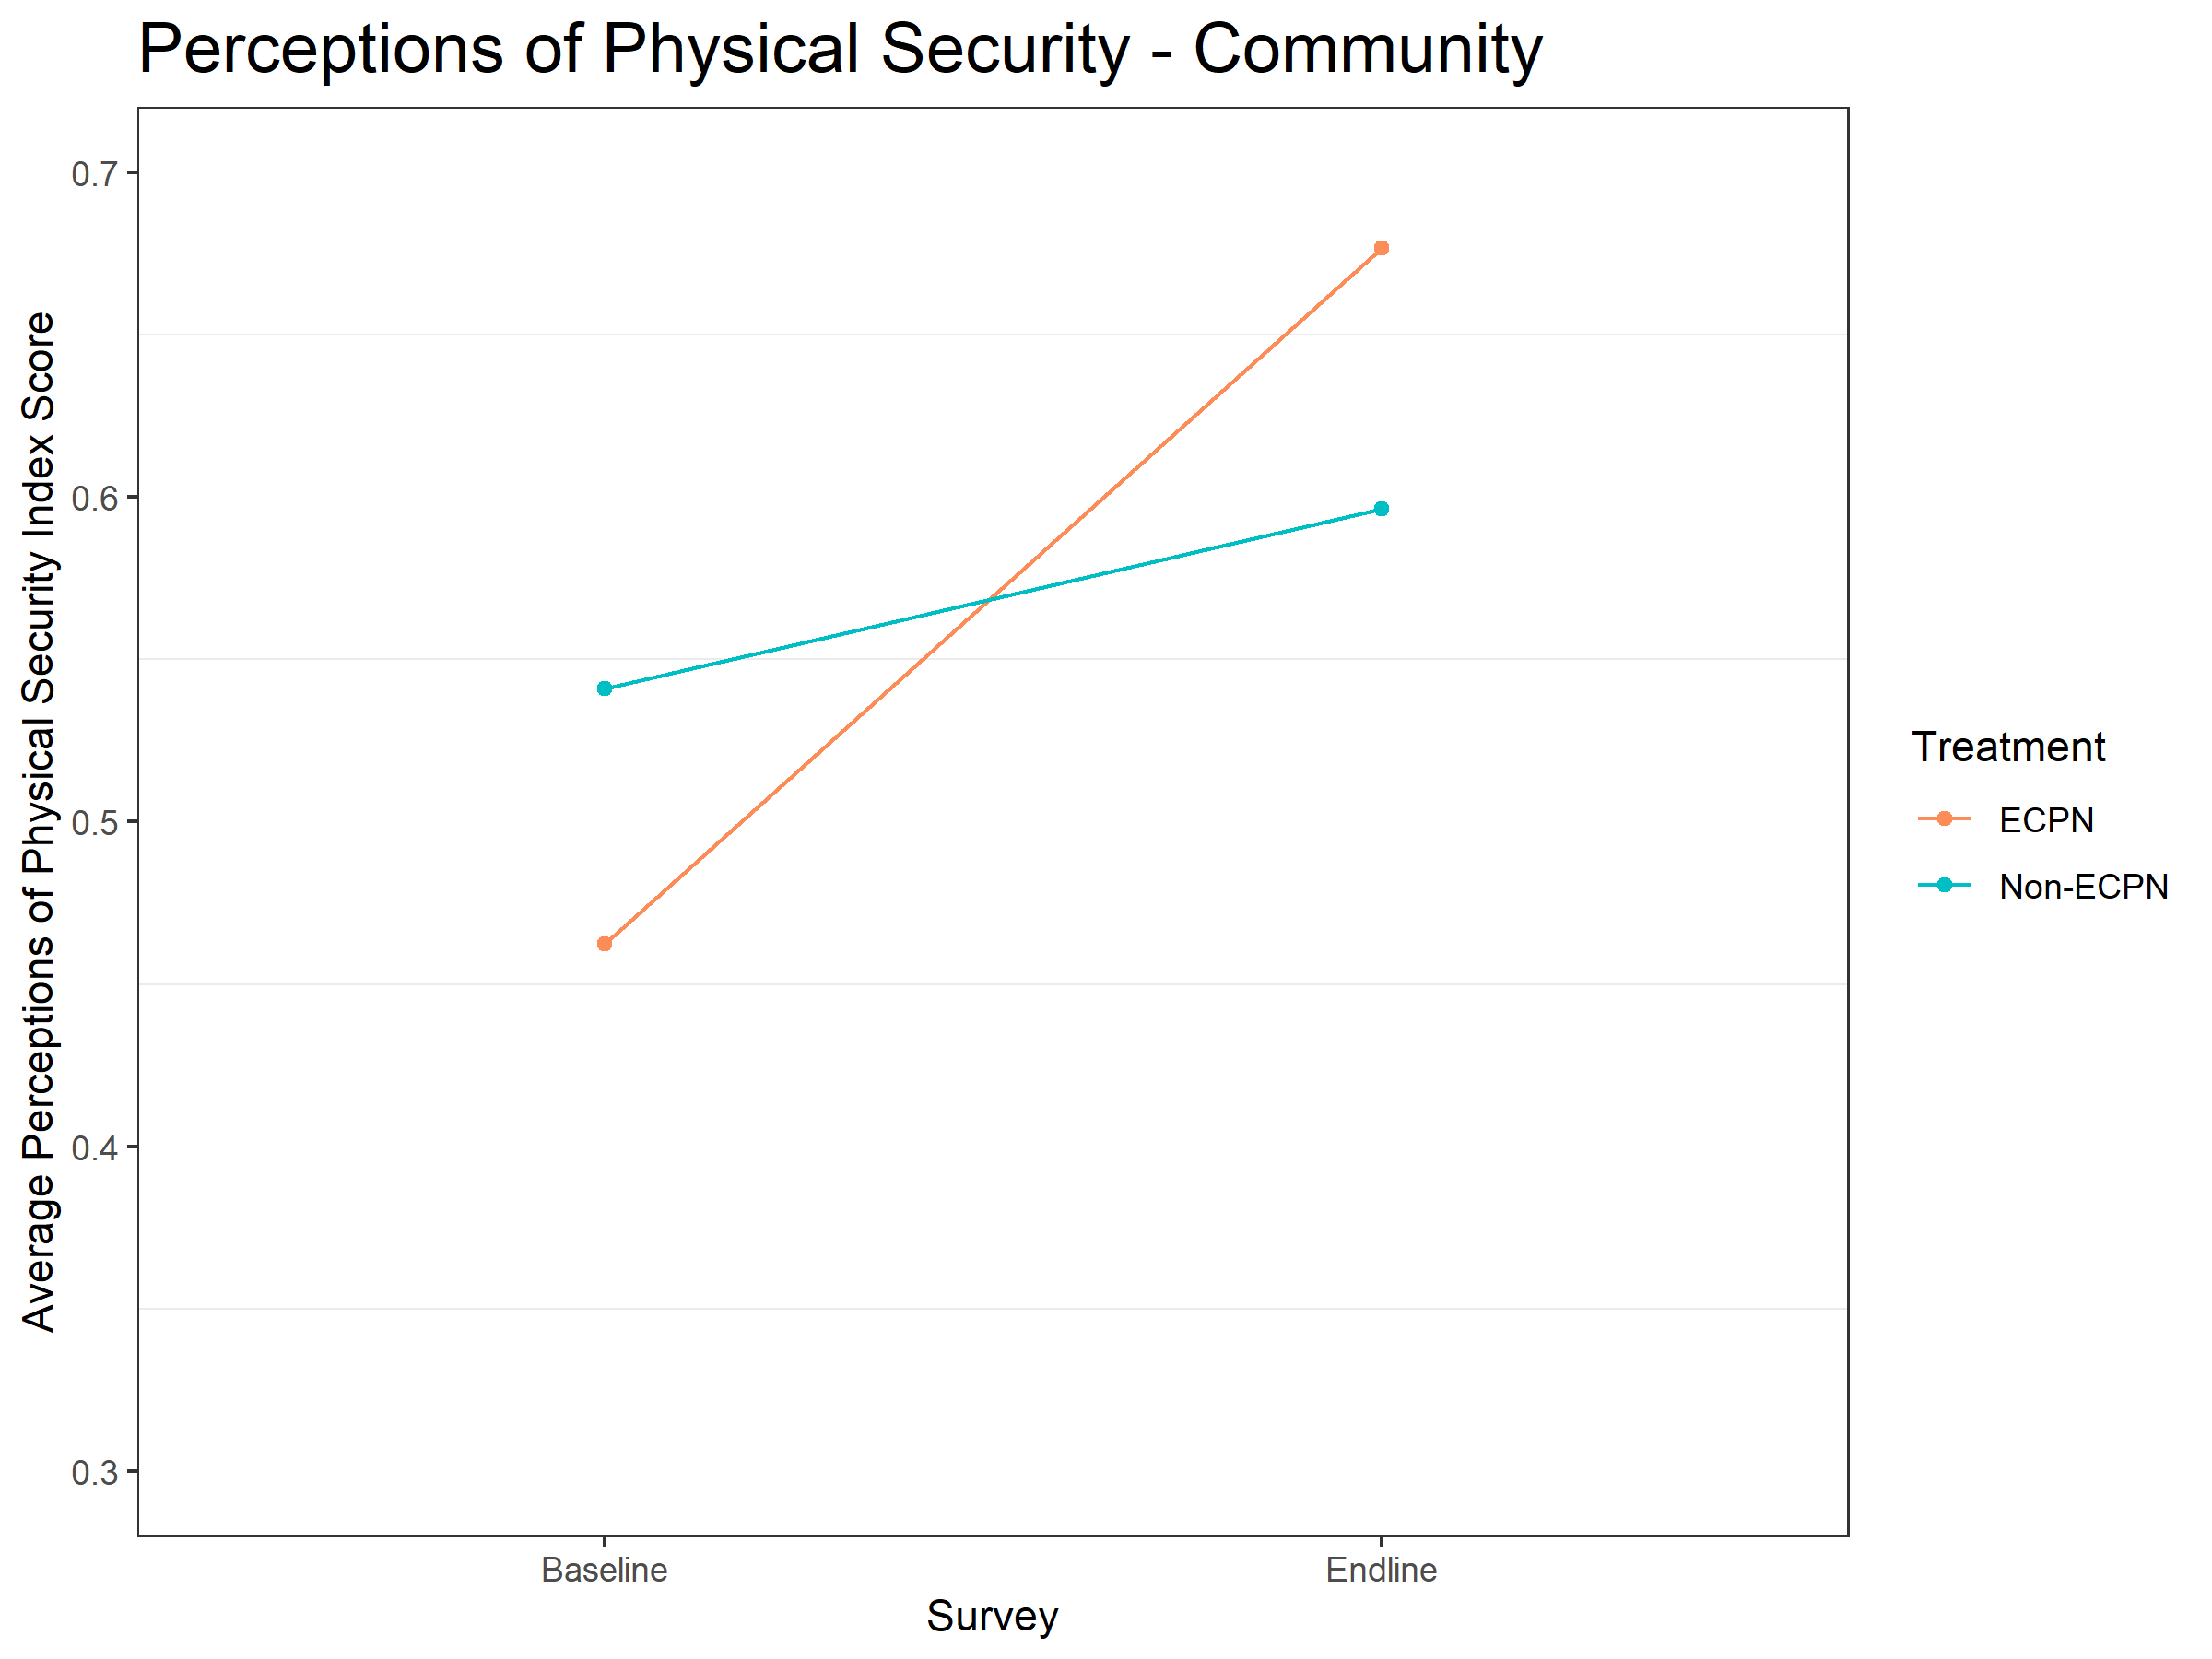
\includegraphics[width=\linewidth]{../figs/inComm_plot.png}
        %\caption{Look at fig 1!}
        \label{fig:fig7}
    \end{minipage}
    \hfill
    \begin{minipage}[b]{.48\textwidth}
        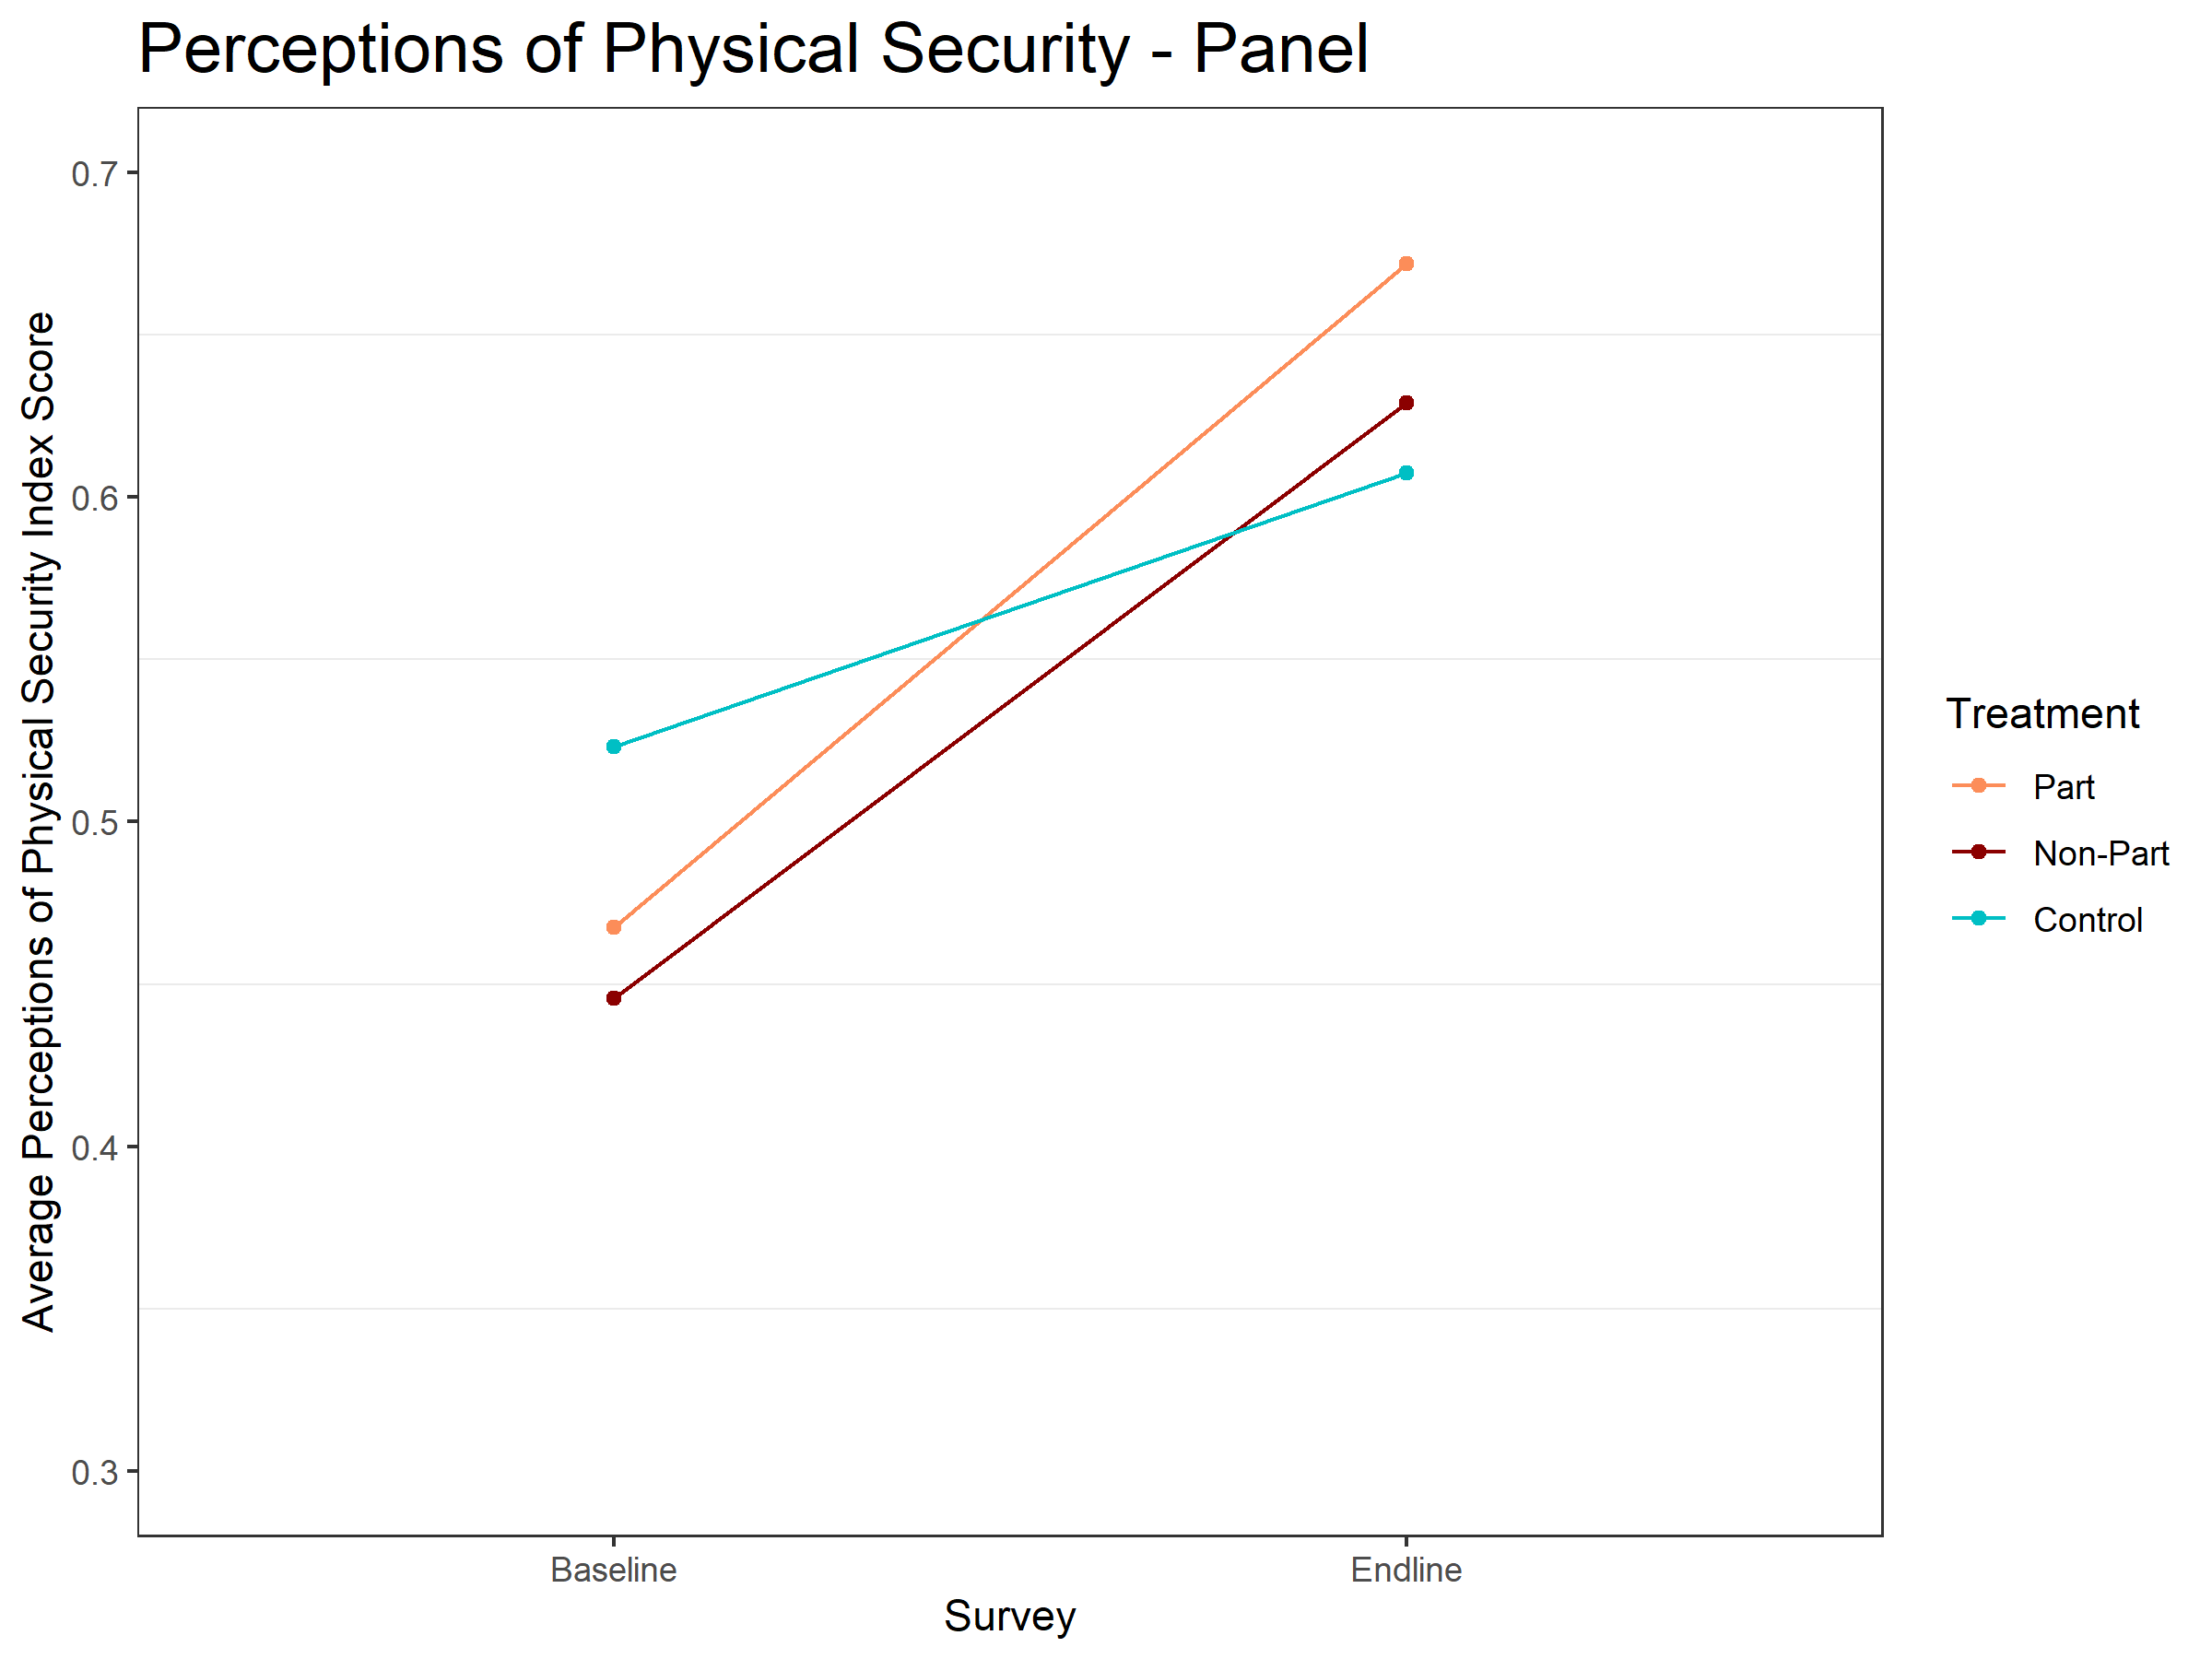
\includegraphics[width=\linewidth]{../figs/inPan_plot.png}
        %\caption{Look at fig 2!}
        \label{fig:fig8}
    \end{minipage}
\end{figure}

Figures 7 and 8 show the effect of ECPN on insecurity. Descriptively,
the insecurity of control communities is largely unchanged from baseline
to endline but insecurity in treatment communities declines
substantially. ECPN communities initially felt more insecure than
control communities but were more secure at the end of the program. ECPN
substantially the security of people in intervention communities.

\hypertarget{placebo-attitudes-about-violence}{%
\subsection{Placebo: attitudes about
violence}\label{placebo-attitudes-about-violence}}

To provide evidence that these survey results are due to intergroup
contact and not due to social desirability bias, we analyze the effect
of ECPN on attitudes about violence. If ECPN affects attitudes about
violence, then we worry that other self-reports were affected by social
desirability bias. If ECPN has no effect on attitudes about violence,
then it is unlikely that other self-reports were affected by social
desirabilty bias.

ECPN has no effect on attitudes about violence in the community-level
data or the individual-level data. {[}note: will add table{]} Table 1
shows two different ways of estimating the effect and two different ways
of measuring attitudes about violence.

\hypertarget{mechanisms-empathy-threat-and-ingroup-expansion}{%
\subsection{Mechanisms: Empathy, Threat, and Ingroup
Expansion}\label{mechanisms-empathy-threat-and-ingroup-expansion}}

Our results suggest that ECPN improved intergroup relations between
farmers and pastoralists. We also undertook an exploratory analysis to
learn the mechanisms through which ECPN affected attitudes. Based on the
literature about contact theory, we looked for evidence that ECPN worked
through empathy and perspective-taking, reduced feelings of threat, and
expansion of the respondent's ingroup to include the former outgroup.

Our exploratory analysis suggests that ECPN may have worked through
increasing empathy. ECPN led to increased empathy in the community and
individual-level analyses. In turn, increased empathy correlated with
improved intergroup affect in the community-level data and with
increases in intergroup affect and intergroup contact at the individual
level. Increased perspective-taking also correlated with intergroup
affect and intergroup contact in both analyses. ECPN may have led to
increased perspective-taking, though not quite to a statistically
significant level. Though this analysis is only exploratory, it suggests
that increased empathy is a plausible mechanism through which ECPN
improved intergroup relations. Because empathy was not randomly
assigned, though, it's equally plausible that ECPN improved intergroup
affect and fostered intergroup contact, and that those outcomes led to
increased empathy.

There is no evidence that ECPN reduced perceptions of threat or expanded
perceptions of the ingroup. ECPN did not effect either survey index, and
the public goods game shows that the treatment group was not better at
coordinating than the control group. Treatment communities donated
\emph{less} to the shared community fund than control communities. At
the individual-level, ECPN participants donated less than
nonparticipants who donated less than respondents in the control group.
This is the opposite pattern of what we would expect if intergroup
contact caused the communities to think of each other as part of one
ingroup. Reduced threat and ingroup expanstion are still plausible
psychological mechanisms -- each correlated strongly with at least one
outcome -- though neither was increased by ECPN.

{[}Table: Rows are mechanisms, columns are outcomes, separated by
community vs individual analyses. Show coefficient (pvalue).{]}


\end{document}
